\documentclass{standalone}
\usepackage{tikz}
\usetikzlibrary{patterns, positioning}


\begin{document}
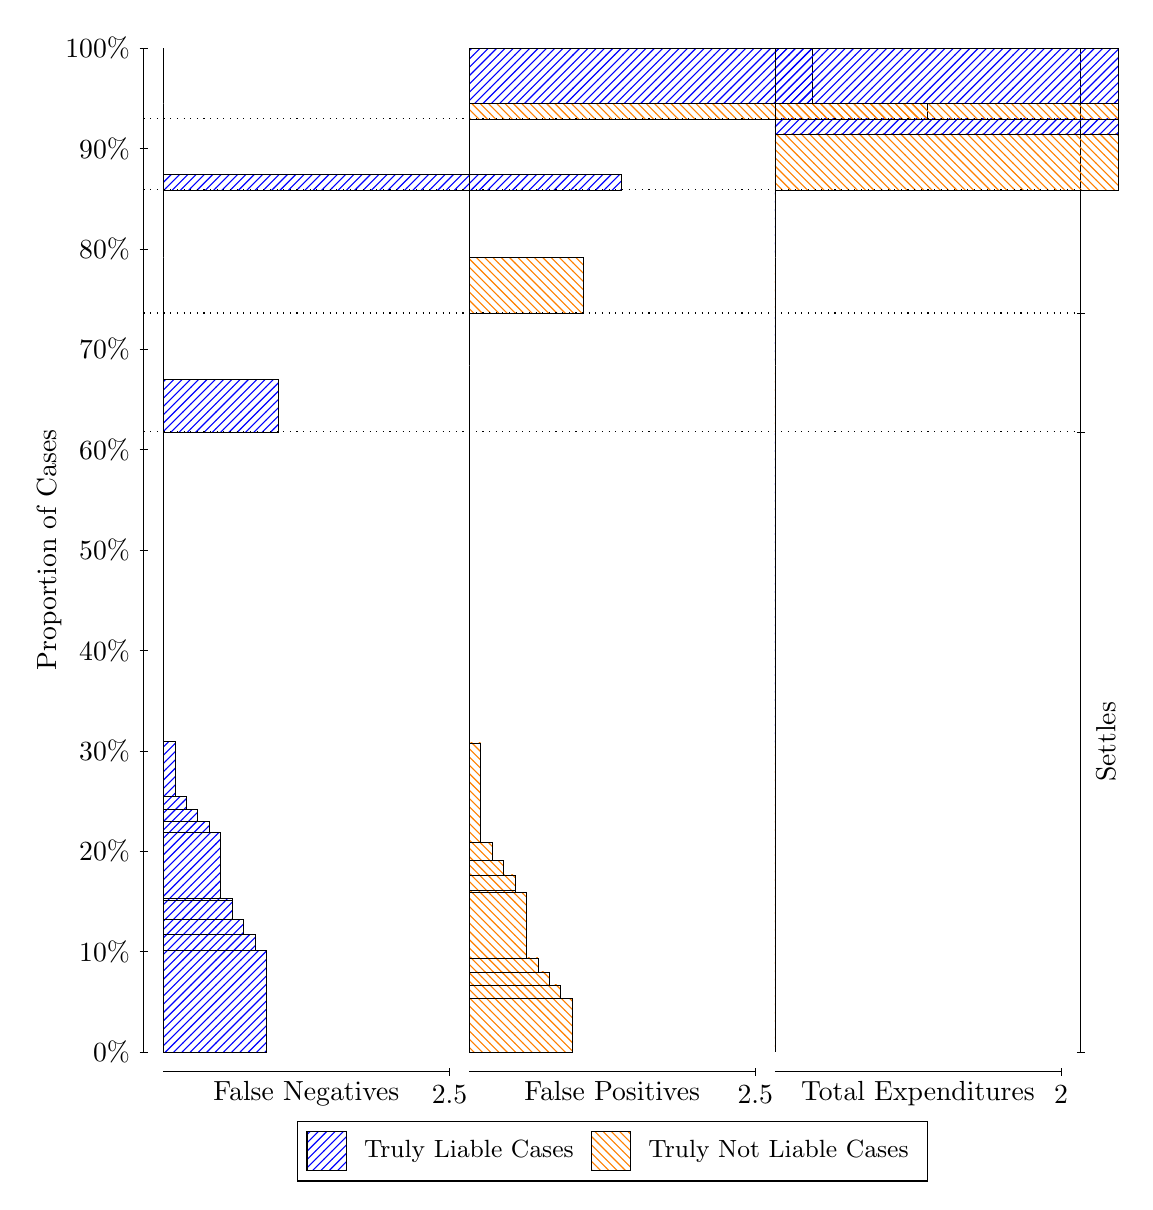
\begin{tikzpicture}
\draw[black, very thin] (1.5,1.75) -- (1.5,14.5);
\node[rotate=90, text=black, anchor=center] at (0.3, 8.125) {Proportion of Cases};
\draw[black, very thin] (1.45,1.75) -- (1.55,1.75);
\node[text=black, anchor=east] at (1.45, 1.75) {0\%};
\draw[black, very thin] (1.45,3.025) -- (1.55,3.025);
\node[text=black, anchor=east] at (1.45, 3.025) {10\%};
\draw[black, very thin] (1.45,4.3) -- (1.55,4.3);
\node[text=black, anchor=east] at (1.45, 4.3) {20\%};
\draw[black, very thin] (1.45,5.575) -- (1.55,5.575);
\node[text=black, anchor=east] at (1.45, 5.575) {30\%};
\draw[black, very thin] (1.45,6.85) -- (1.55,6.85);
\node[text=black, anchor=east] at (1.45, 6.85) {40\%};
\draw[black, very thin] (1.45,8.125) -- (1.55,8.125);
\node[text=black, anchor=east] at (1.45, 8.125) {50\%};
\draw[black, very thin] (1.45,9.4) -- (1.55,9.4);
\node[text=black, anchor=east] at (1.45, 9.4) {60\%};
\draw[black, very thin] (1.45,10.675) -- (1.55,10.675);
\node[text=black, anchor=east] at (1.45, 10.675) {70\%};
\draw[black, very thin] (1.45,11.95) -- (1.55,11.95);
\node[text=black, anchor=east] at (1.45, 11.95) {80\%};
\draw[black, very thin] (1.45,13.225) -- (1.55,13.225);
\node[text=black, anchor=east] at (1.45, 13.225) {90\%};
\draw[black, very thin] (1.45,14.5) -- (1.55,14.5);
\node[text=black, anchor=east] at (1.45, 14.5) {100\%};

\draw[black, very thin] (13.4,1.75) -- (13.4,14.5);
\draw[black, very thin] (13.35,1.75) -- (13.45,1.75);
\node[anchor=west] at (13.35, 1.75) {};
\draw[black, very thin] (13.35,9.6256) -- (13.45,9.6256);
\node[anchor=west] at (13.35, 9.6256) {};
\draw[black, very thin] (13.35,11.135) -- (13.45,11.135);
\node[anchor=west] at (13.35, 11.135) {};
\draw[black, very thin] (13.35,12.699) -- (13.45,12.699);
\node[anchor=west] at (13.35, 12.699) {};
\draw[black, very thin] (13.35,13.601) -- (13.45,13.601);
\node[anchor=west] at (13.35, 13.601) {};
\draw[black, very thin] (13.35,14.5) -- (13.45,14.5);
\node[anchor=west] at (13.35, 14.5) {};

\draw[black, very thin, pattern color=blue, pattern=north east lines] (1.75,1.75) rectangle (3.058,3.043);
\draw[black, very thin, pattern color=blue, pattern=north east lines] (1.75,3.043) rectangle (2.9127,3.2439);
\draw[black, very thin, pattern color=blue, pattern=north east lines] (1.75,3.2439) rectangle (2.7673,3.4371);
\draw[black, very thin, pattern color=blue, pattern=north east lines] (1.75,3.4371) rectangle (2.622,3.6795);
\draw[black, very thin, pattern color=blue, pattern=north east lines] (1.75,3.6795) rectangle (2.622,3.703);
\draw[black, very thin, pattern color=blue, pattern=north east lines] (1.75,3.703) rectangle (2.4767,4.5404);
\draw[black, very thin, pattern color=blue, pattern=north east lines] (1.75,4.5404) rectangle (2.3313,4.6826);
\draw[black, very thin, pattern color=blue, pattern=north east lines] (1.75,4.6826) rectangle (2.186,4.828);
\draw[black, very thin, pattern color=blue, pattern=north east lines] (1.75,4.828) rectangle (2.0407,4.997);
\draw[black, very thin, pattern color=blue, pattern=north east lines] (1.75,4.997) rectangle (1.8953,5.6992);
\draw[black, very thin, pattern color=orange, pattern=north west lines] (1.75,5.6992) rectangle (1.75,9.6256);
\draw[black, very thin, pattern color=blue, pattern=north east lines] (1.75,9.6256) rectangle (3.2033,10.29);
\draw[black, very thin, pattern color=orange, pattern=north west lines] (1.75,10.29) rectangle (1.75,11.135);
\draw[black, very thin, pattern color=orange, pattern=north west lines] (1.75,11.135) rectangle (1.75,11.837);
\draw[black, very thin, pattern color=blue, pattern=north east lines] (1.75,11.837) rectangle (1.75,12.699);
\draw[black, very thin, pattern color=blue, pattern=north east lines] (1.75,12.699) rectangle (7.5633,12.891);
\draw[black, very thin, pattern color=orange, pattern=north west lines] (1.75,12.891) rectangle (1.75,13.601);
\draw[black, very thin, pattern color=orange, pattern=north west lines] (1.75,13.601) rectangle (1.75,13.793);
\draw[black, very thin, pattern color=blue, pattern=north east lines] (1.75,13.793) rectangle (1.75,14.5);
\draw[black, very thin, pattern color=orange, pattern=north west lines] (5.6333,1.75) rectangle (6.9413,2.429);
\draw[black, very thin, pattern color=orange, pattern=north west lines] (5.6333,2.429) rectangle (6.796,2.6007);
\draw[black, very thin, pattern color=orange, pattern=north west lines] (5.6333,2.6007) rectangle (6.6507,2.7668);
\draw[black, very thin, pattern color=orange, pattern=north west lines] (5.6333,2.7668) rectangle (6.5053,2.9447);
\draw[black, very thin, pattern color=orange, pattern=north west lines] (5.6333,2.9447) rectangle (6.36,3.7763);
\draw[black, very thin, pattern color=orange, pattern=north west lines] (5.6333,3.7763) rectangle (6.2147,3.8024);
\draw[black, very thin, pattern color=orange, pattern=north west lines] (5.6333,3.8024) rectangle (6.2147,3.9985);
\draw[black, very thin, pattern color=orange, pattern=north west lines] (5.6333,3.9985) rectangle (6.0693,4.1799);
\draw[black, very thin, pattern color=orange, pattern=north west lines] (5.6333,4.1799) rectangle (5.924,4.4102);
\draw[black, very thin, pattern color=orange, pattern=north west lines] (5.6333,4.4102) rectangle (5.7787,5.6764);
\draw[black, very thin, pattern color=blue, pattern=north east lines] (5.6333,5.6764) rectangle (5.6333,9.6256);
\draw[black, very thin, pattern color=orange, pattern=north west lines] (5.6333,9.6256) rectangle (5.6333,10.47);
\draw[black, very thin, pattern color=blue, pattern=north east lines] (5.6333,10.47) rectangle (5.6333,11.135);
\draw[black, very thin, pattern color=orange, pattern=north west lines] (5.6333,11.135) rectangle (7.0867,11.837);
\draw[black, very thin, pattern color=blue, pattern=north east lines] (5.6333,11.837) rectangle (5.6333,12.699);
\draw[black, very thin, pattern color=orange, pattern=north west lines] (5.6333,12.699) rectangle (5.6333,13.41);
\draw[black, very thin, pattern color=blue, pattern=north east lines] (5.6333,13.41) rectangle (5.6333,13.601);
\draw[black, very thin, pattern color=orange, pattern=north west lines] (5.6333,13.601) rectangle (11.447,13.793);
\draw[black, very thin, pattern color=blue, pattern=north east lines] (5.6333,13.793) rectangle (9.9933,14.5);
\draw[black, very thin, pattern color=orange, pattern=north west lines] (9.5167,1.75) rectangle (9.5167,5.6764);
\draw[black, very thin, pattern color=blue, pattern=north east lines] (9.5167,5.6764) rectangle (9.5167,9.6256);
\draw[black, very thin, pattern color=orange, pattern=north west lines] (9.5167,9.6256) rectangle (9.5167,10.47);
\draw[black, very thin, pattern color=blue, pattern=north east lines] (9.5167,10.47) rectangle (9.5167,11.135);
\draw[black, very thin, pattern color=orange, pattern=north west lines] (9.5167,11.135) rectangle (9.5167,11.837);
\draw[black, very thin, pattern color=blue, pattern=north east lines] (9.5167,11.837) rectangle (9.5167,12.699);
\draw[black, very thin, pattern color=orange, pattern=north west lines] (9.5167,12.699) rectangle (13.877,13.41);
\draw[black, very thin, pattern color=blue, pattern=north east lines] (9.5167,13.41) rectangle (13.877,13.601);
\draw[black, very thin, pattern color=orange, pattern=north west lines] (9.5167,13.601) rectangle (13.877,13.793);
\draw[black, very thin, pattern color=blue, pattern=north east lines] (9.5167,13.793) rectangle (13.877,14.5);
\draw[black, dotted] (1.5,9.6256) -- (13.4,9.6256);
\draw[black, dotted] (1.5,11.135) -- (13.4,11.135);
\draw[black, dotted] (1.5,12.699) -- (13.4,12.699);
\draw[black, dotted] (1.5,13.601) -- (13.4,13.601);
\draw[black, very thin] (1.75,1.5) -- (5.3833,1.5);
\node[text=black, anchor=north] at (3.5667, 1.5) {False Negatives};
\draw[black, very thin] (5.3833,1.45) -- (5.3833,1.55);
\node[text=black, anchor=north] at (5.3833, 1.45) {2.5};

\draw[black, very thin] (5.6333,1.5) -- (9.2667,1.5);
\node[text=black, anchor=north] at (7.45, 1.5) {False Positives};
\draw[black, very thin] (9.2667,1.45) -- (9.2667,1.55);
\node[text=black, anchor=north] at (9.2667, 1.45) {2.5};

\draw[black, very thin] (9.5167,1.5) -- (13.15,1.5);
\node[text=black, anchor=north] at (11.333, 1.5) {Total Expenditures};
\draw[black, very thin] (13.15,1.45) -- (13.15,1.55);
\node[text=black, anchor=north] at (13.15, 1.45) {2};

\node[text=black, centered, rotate=90] at (13.72, 5.6878) {Settles};





\draw (7.449999999999999,1.5) node[draw=none] (baseCoordinate) {};
\begin{scope}[align=center]
        \matrix[scale=0.5, draw=black, below=0.5cm of baseCoordinate, nodes={draw}, column sep=0.1cm]{
            \node[rectangle, draw, minimum width=0.5cm, minimum height=0.5cm, pattern color=blue, pattern=north east lines] {}; &
            \node[draw=none, font=\small, text=black] (B) {Truly Liable Cases}; &
            \node[rectangle, draw, minimum width=0.5cm, minimum height=0.5cm, pattern color=orange, pattern=north west lines] {}; &
            \node[draw=none, font=\small, text=black] (B) {Truly Not Liable Cases}; \\
            };
\end{scope}

\end{tikzpicture}
\end{document}